\documentclass[a4paper,11pt]{article}

\usepackage[utf8]{inputenc}
\usepackage[english]{babel}

\usepackage{amsmath}

% Code highligting
% \usepackage{minted}
\usepackage[outputdir=output/tex]{minted} % iom min makefile

\newenvironment{longlisting}{\captionsetup{type=listing}}{}
% \renewcommand\listoflistingscaption{Källkod....}
\renewcommand\listoflistingscaption{List of source codes}
%\setmintedinline[sql]{breaklines=true,breakanywhere=true} % necessary for breakanywhere to work later on.

\usepackage{graphicx}
\usepackage{pgf}
\usepackage{wrapfig}
\usepackage[font=footnotesize,labelfont=bf,skip=1pt]{caption}
\usepackage{subcaption}

\usepackage{pgfplots}
\pgfplotsset{compat=1.18}

\usepackage{pgfplotstable}
\usepackage{booktabs}

% Spacing
\usepackage{titlesec}
%\titlespacing*{\section}{0pt}{2ex plus 1ex minus .2ex}{1ex plus .2ex}
%\titlespacing*{\subsection}{0pt}{1ex plus 1ex minus .2ex}{1ex plus .2ex}

\usepackage{hyperref}

\begin{document}
\title{
    Generating a Mandelbrot Image
\\\small{Programmering II, ID1019, VT24 P1}
}
\author{Vincent Ferrigan \href{mailto:ferrigan@kth.se}{ferrigan@kth.se}}

\date{\today}
\maketitle

\section*{Introduction}
\label{sec:introduction}
This assignment is about implementing a Mandelbrot set generator in
Elixir, which will ultimately produce an image of the Mandelbrot set. 
The steps outlined in the document are as follows:
\begin{enumerate}
    \item Complex Numbers Module: Implement a module to handle complex numbers,
    including functions for creating new complex numbers, adding two complex
    numbers, squaring a complex number, and finding the absolute value of a
    complex number.
    \item Mandelbrot Computation Module: Implement the core logic to determine
    if a given complex number belongs to the Mandelbrot set based on a maximum
    iteration depth.
    This involves calculating the sequence of complex numbers
    and checking if their absolute values exceed a certain threshold before
    reaching the maximum number of iterations.
    \item Image Generation: Using the PPM module to generate an image file from
    the calculated data.
    This module was given by the course.
    \item Color Module: Implement a module to convert the depth (number of
    iterations) to RGB color values, which will be used to color the Mandelbrot
    image.
    \item Mandelbrot Set Generation: Combine all the above to generate the
    Mandelbrot set over a defined area and resolution, and save this as an image
    using the PPM module.
\end{enumerate}
This assignment is based on the instruction
\href{https://people.kth.se/~johanmon/courses/id1019/seminars/mandel/mandel.pdf}{'Generating a Mandelbrot Image'}
by course examiner Johan Montelius.
The Mix-project for this assignment, including all relative functions, Unit-test and images can be found on GitHub:
\href{https://github.com/VincentFerrigan/kth-id1019-programming-ii/tree/main/tasks/7/mandelbrot}{Repo Programming II - Mandelbrot}% TODO FUNKAR DEN? ÄNDRA NAMN

\section*{Methods}\label{sec:methods}
\subsection*{Literature Study}
\label{subsec:literaturestudy}
Elixir-syntax and similar topics were acquired
from both the
\href{https://elixir-lang.org/docs.html}{Elixir official documentation}
and the free Elixir Tutorial
\href{https://elixirschool.com/en}{Elixir School
website}.
The author also relied on textbooks found on
\href{https://learning.oreilly.com}{O'Reilly Media},
especially Brute Tate's
\href{https://learning.oreilly.com/library/view/programmer-passport-elixir/9781680509649/}{Programmer Passport: Elixir}.

\subsubsection*{Tools and packages}
\label{subsec:tools}
All code was written in \emph{IntelliJ IDEA}.
Quick-fixes and editing was, however, done in \emph{Vim}.
\emph{GIT} and \emph{GitHub} were used for version control.
Tests were performed with Elixir's built-in test framework \emph{ExUnit.}
The report was written in \LaTeX and the generated ppm-files were converted by a python script.
% For exploration and benchmarking, the interactive environment and notebook
% \href{https://livebook.dev/}{\emph{Livebook}}
% was heavily used.

\subsubsection*{Test Driven Development}\label{sec:ttd}
The development was an iterative approach with ''trail and errors''.
The author practiced
\href{https://www.elixirwiki.com/wiki/Test-Driven_Development_in_Elixir}{Test Driven Development}
(TDD).
The basic steps follow the \emph{Red-Green-Refactor cycle};
writing failing tests (Red), make them pass (Green),
and finally refactor the code.
For example, before creating all the necessary functions for the
\mintinline{elixir}{Cmplx} module,
one can first write a couple of test cases, as illustrated in the test-example below.
%TODO.
\inputminted[
    label=CMPLX TESTS,
    firstline=5,
    lastline=8,
    xleftmargin=-3mm,  % Adjust this value as needed
    fontsize=\footnotesize,
]{elixir}{../test/cmplx_test.exs}
\noindent The
\mintinline{elixir}{sqr/1} function is supposed to square the complex number
$1 + 2i$, where $i$
is the imaginary unit, with the formula for squaring binomials
$(a + bi)^2$ -- which is \(a^2+2abi-b^2\), noting that $i^2 = -1$.
\noindent So for $1 + 2i$:
\[(1 + 2i)^2 = 1^2 + 2 \cdot 1 \cdot 2i + (2i)^2 = 1 + 4i - 4 = -3 + 4i\]
Which the test above is to assert.
The function was therefore created as follows:
\inputminted[
    label=sqr/1,
    firstline=47,
    lastline=50,
    xleftmargin=-3mm,  % Adjust this value as needed
    fontsize=\footnotesize,
]{elixir}{../lib/cmplx.ex}

\clearpage
\subsection*{Complex Numbers Module}
\label{subsec:cmplx}
The module
\mintinline{elixir}{Cmplx},
is designed to handle basic operations with complex numbers.
\inputminted[
    label=cpx,
    firstline=12,
    lastline=12,
    xleftmargin=-3mm,  % Adjust this value as needed
    fontsize=\footnotesize,
]{elixir}{../lib/cmplx.ex}
\noindent These numbers are represented as tuples,
\mintinline{elixir}{{:cpx, real, imag}}, where
\mintinline{elixir}{real} is the real part and
\mintinline{elixir}{imag} is the imaginary part of the complex number.
The
\mintinline{elixir}{:cpx}
tag is used to explicitly identify the tuple as representing a complex number.
\mintinline{elixir}{Cmplx.new/2}
creates a new complex number, given its real and imaginary parts
while
\mintinline{elixir}{Cmplx.add/2} adds two complex numbers.
The addition is performed by adding the real parts and the imaginary parts separately.
\inputminted[
    label=new/2,
    firstline=25,
    lastline=26,
    xleftmargin=-3mm,  % Adjust this value as needed
    fontsize=\footnotesize,
]{elixir}{../lib/cmplx.ex}
\inputminted[
    label=iex new/2,
    firstline=22,
    lastline=23,
    xleftmargin=-10mm,  % Adjust this value as needed
    fontsize=\footnotesize,
]{elixir}{../lib/cmplx.ex}
\inputminted[
    label=add/2,
    firstline=35,
    lastline=38,
    xleftmargin=-3mm,  % Adjust this value as needed
    fontsize=\footnotesize,
]{elixir}{../lib/cmplx.ex}
\inputminted[
    label=iex add/2,
    firstline=32,
    lastline=33,
    xleftmargin=-10mm,  % Adjust this value as needed
    fontsize=\footnotesize,
]{elixir}{../lib/cmplx.ex}
The function for squaring complex numbers,
\mintinline{elixir}{Cmplx.sqr/1},
was demonstrated in the previous subsection above.
The last function,
\mintinline{elixir}{Cmplx.abs/1},
operates on a single complex number.
It calculates the absolute
value (magnitude) of a complex number -- i.e. the distance of the complex number
from the origin in the complex plane.
\inputminted[
    label=abs/1,
    firstline=59,
    lastline=60,
    xleftmargin=-3mm,  % Adjust this value as needed
    fontsize=\footnotesize,
]{elixir}{../lib/cmplx.ex}
\inputminted[
    label=iex abs/1,
    firstline=56,
    lastline=57,
    xleftmargin=-10mm,  % Adjust this value as needed
    fontsize=\footnotesize,
]{elixir}{../lib/cmplx.ex}

%This value is essential for determining the escape time of points in the Mandelbrot set calculation.
%The absolute value is used to test if the iterative computation should terminate.
\subsection*{Mandelbrot Computation Module}
\label{subsec:brot}
The
\mintinline{elixir}{Brot} module
focuses on the computation aspect.
It determines whether a point belongs to the Mandelbrot set
based on the iteration depth and complex number calculations.
It implements the core algorithm that performs the iterative calculation
to check if a given complex number escapes the set within a certain number
of iterations.

The Mandelbrot set is defined by a simple mathematical formula applied to complex numbers.
For each point $c$ in the complex plane, we iterate the formula
\(z_{n+1} = z^2_n + c\), starting with $z_{0}=0$.
A point $c$ is considered part of the Mandelbrot set if,
after an infinite number of iterations, the value of
$z$ does not escape to infinity.

In practice, we cannot iterate infinitely,
so we set a maximum number of iterations
\mintinline{elixir}{`max_iterations`} to decide whether
$z$ escapes or not.
\inputminted[
    label=Brot.mandelbrot/1,
    firstline=41,
    lastline=59,
    xleftmargin=-3mm,  % Adjust this value as needed
    fontsize=\footnotesize,
]{elixir}{../lib/brot.ex}

\noindent As shown in the helper function
\mintinline{elixir}{perform_iteration},
if $|z|$ becomes greater than our threshold $2$
before hitting the maximum iteration count, we consider
$c$ not part of the set.
The number of iterations it takes for
$z$ to escape gives us a way to color points not in the set,
creating the beautiful fractal images associated with the Mandelbrot set.

\subsection*{Color Module}
\label{subsec:color}
The
\mintinline{elixir}{Color} module is designed to map numerical values,
specifically the number of iterations it takes for a point to escape
(or be determined outside) the Mandelbrot set, to color values.
%This mapping is essential for visualizing the Mandelbrot set,
%where different colors can represent the ''speed'' at which points escape
%to infinity, providing a visual cue to the complexity and boundary of the set.
The primary funciton
\mintinline{elixir}{Color.convert/3}
takes the iteration count for a specific point,
\mintinline{elixir}{depth}, and
\mintinline{elixir}{max}, the maximum number of iterations used in the Mandelbrot calculation.
The iteration count,
\mintinline{elixir}{depth}, is a measure of how quickly points escape the boundary of the Mandelbrot set.

Based of the value of
\mintinline{elixir}{depth} relative to
\mintinline{elixir}{max},
the function calculates color values (RGB) that represent the point's behavior under iteration.
The result is a color value, represented as an, RGB tuple, that is used to color a pixel in the final image.

The comments provided for the helper functions are extensive enough to be self-explanatory.
See
\href{https://github.com/VincentFerrigan/kth-id1019-programming-ii/tree/main/tasks/7/mandelbrot/lib/color.ex}{code (lib/color.ex)}.
%\inputminted[
%    label=Color.convert/3,
%    firstline=21,
%    lastline=30,
%    xleftmargin=-3mm,  % Adjust this value as needed
%    fontsize=\footnotesize,
%]{elixir}{../lib/color.ex}
%\inputminted[
%    label=Color.red/2,
%    firstline=33,
%    lastline=55,
%    xleftmargin=-3mm,  % Adjust this value as needed
%    fontsize=\footnotesize,
%]{elixir}{../lib/color.ex}
%\inputminted[
%    label=Color-comment,
%    firstline=92,
%    lastline=92,
%    xleftmargin=-3mm,  % Adjust this value as needed
%    fontsize=\footnotesize,
%]{elixir}{../lib/color.ex}

\subsection*{Mandelbrot Set Generation}
\label{subsec:generator}
The
\mintinline{elixir}{MandelbrotGenerator} module provides the functionality for generating and visualizing the Mandelbrot set
within a specified viewport and resolution.
It is designed to calculate the Mandelbrot set for a given area in the complex plane,
determined by the viewport's center
(\mintinline{elixir}{x_center},
 \mintinline{elixir}{y_center}), zoom level
(\mintinline{elixir}{scale}), and the image resolution
(\mintinline{elixir}{width},
\mintinline{elixir}{height}).
It iterates over each pixel, computes whether it belongs to the Mandelbrot set within a specified depth
(\mintinline{elixir}{max_iterations}), and applies a color scheme
(\mintinline{elixir}{color_scheme}) based on the iteration count for each point.
\inputminted[
    label=MandelbrotGenerator.mandelbrot/7,
    firstline=30,
    lastline=62,
    xleftmargin=-3mm,  % Adjust this value as needed
    fontsize=\footnotesize,
]{elixir}{../lib/mandelbrotgenerator.ex}
\noindent Note that an asynchronous task is initiated for each row of the image using
\mintinline{elixir}{Task.async/1}.
This divides the image generation into parallel tasks,
where each task is responsible for computing the color values of a single row in the image.

\section*{Result}
\label{sec:result}
A
\mintinline{elixir}{MandelDemo} module was created to facilitate the generation and saving of Mandelbrot set images
with customizable parameters and color mappings.
The module prompts the user for several inputs that define the properties of the Mandelbrot set image to be generated.
\begin{figure}[h!]
    \centering
    
\includegraphics[width=0.6\textwidth]{../images/mb_large_green_x-2.3_y1.1_xn0.0008.png}
    \caption{Visualization of the Mandelbrot set.}
    \label{fig:mandelbrot1}
\end{figure}
\begin{figure}[h!]
    \centering
    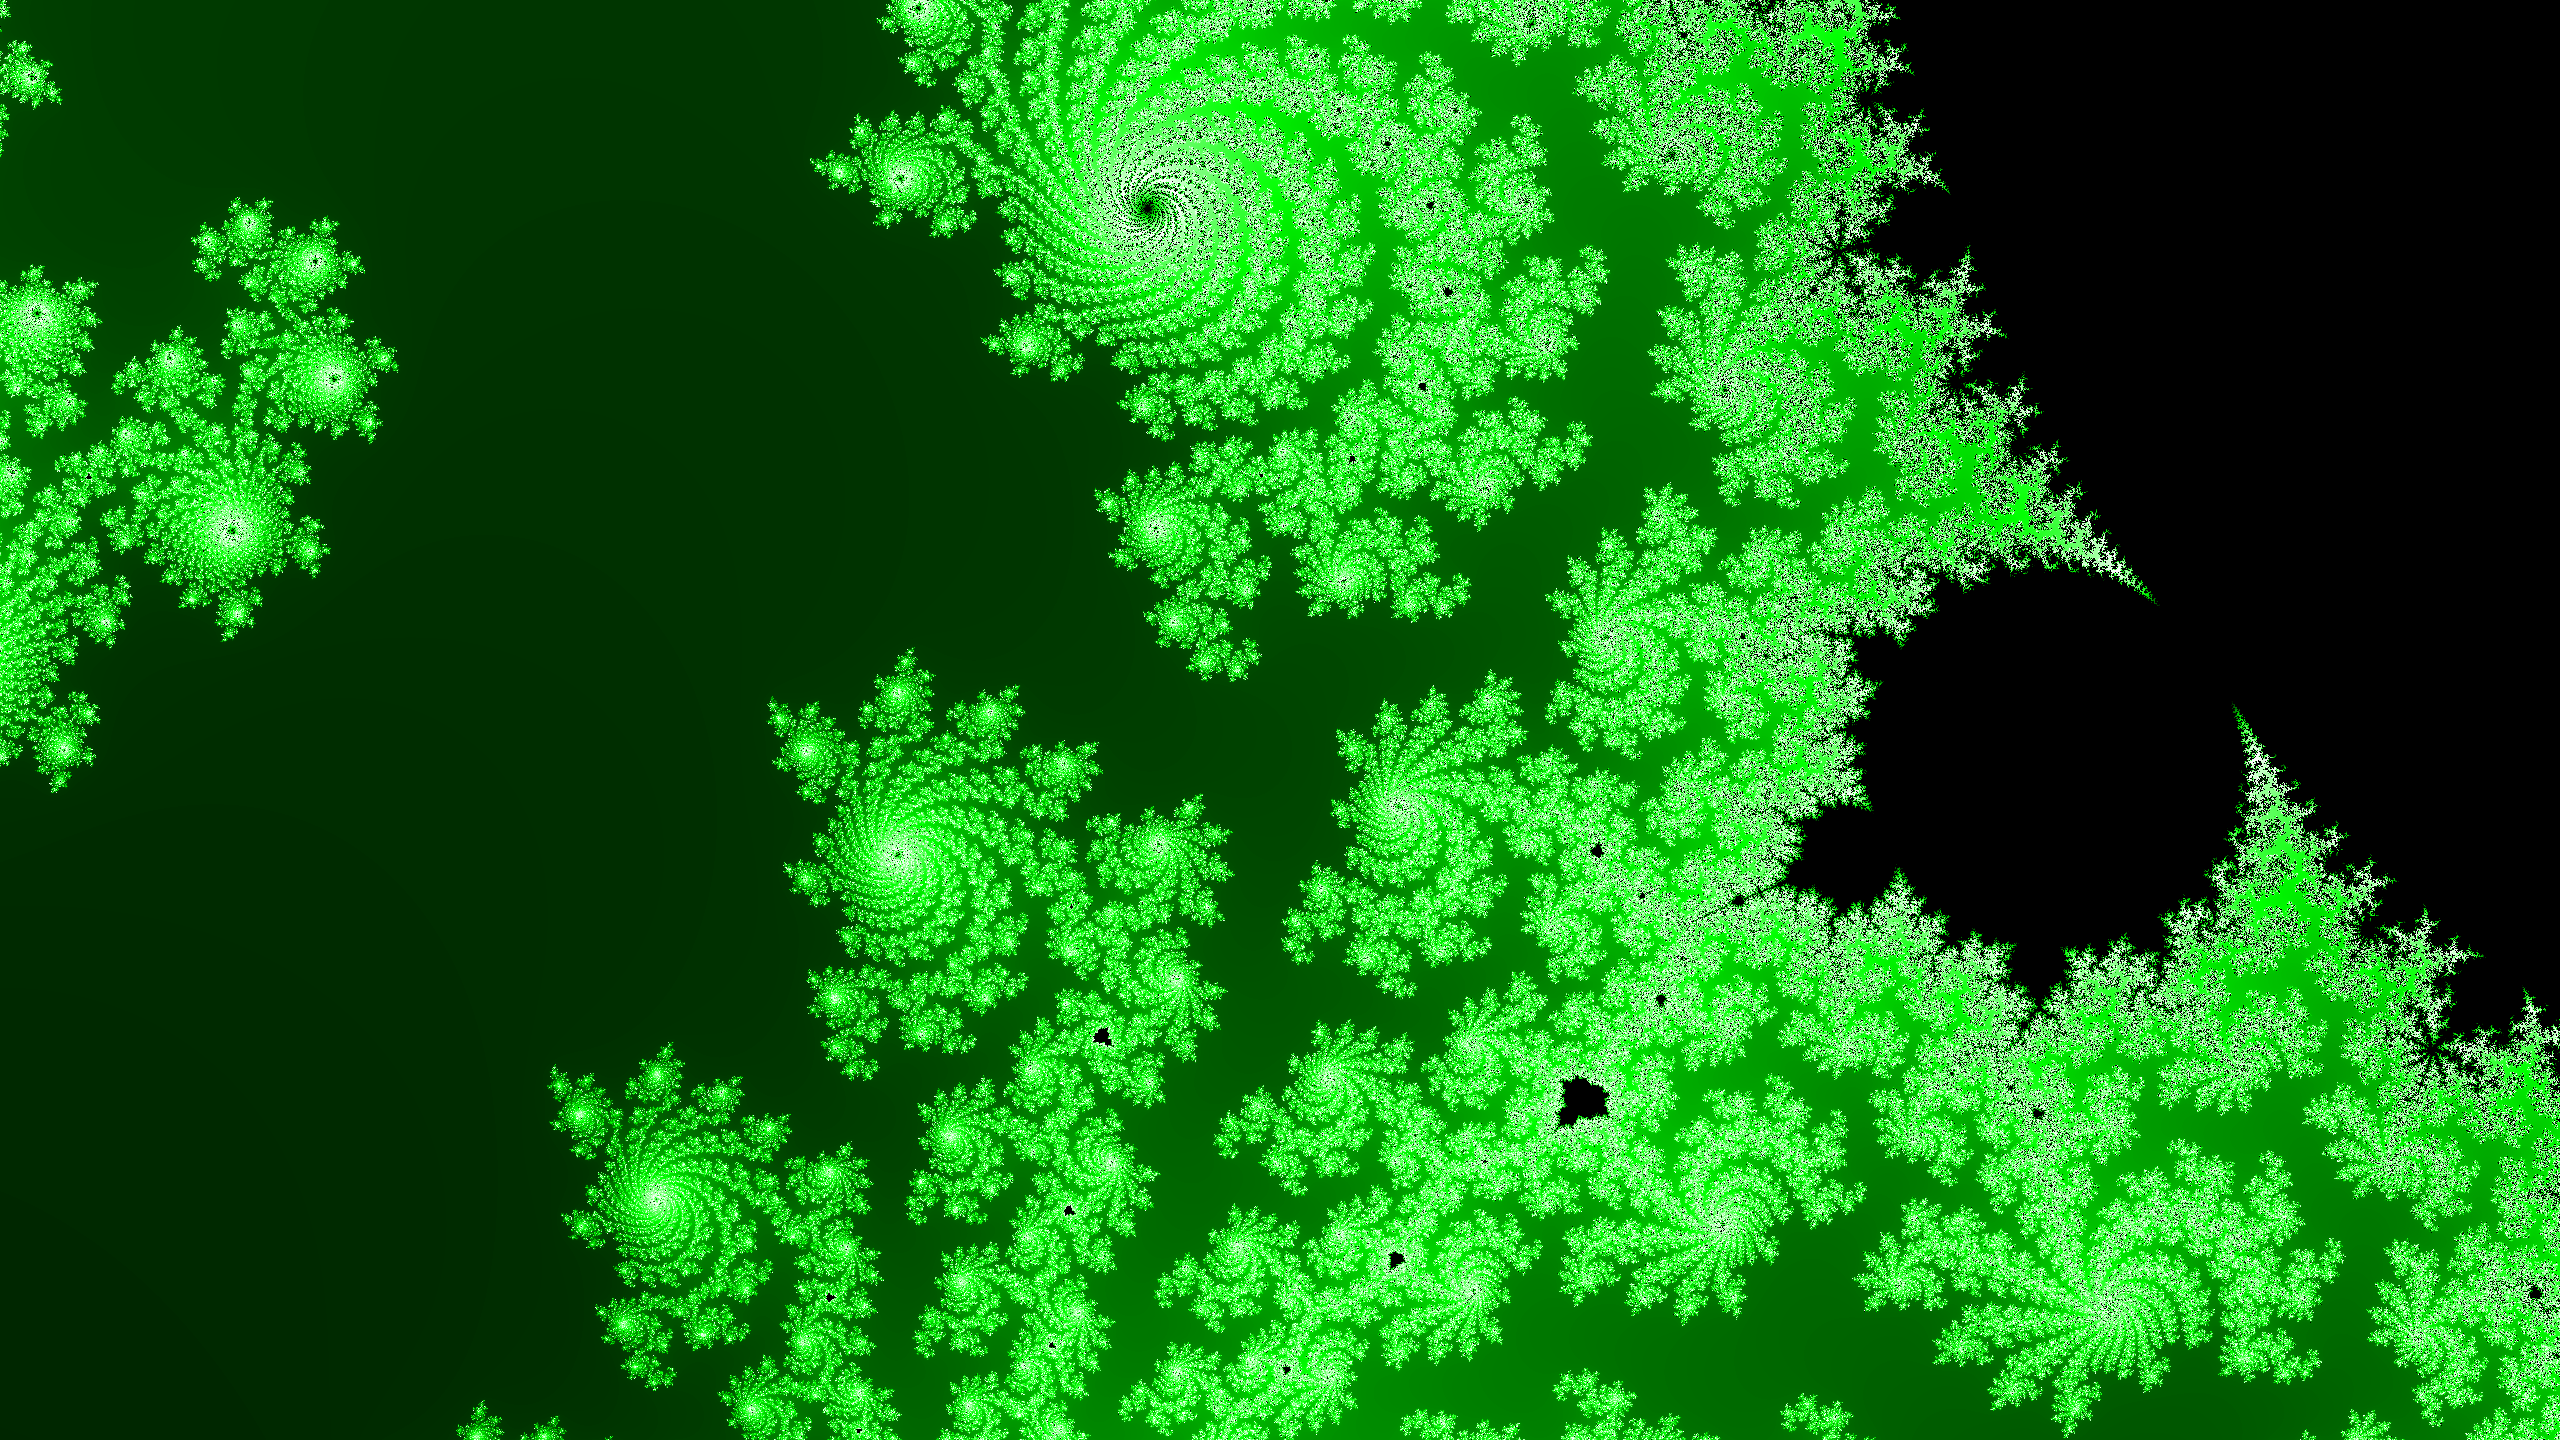
\includegraphics[width=0.6\textwidth]{../images/mb_large_green_x1.0e-5_y0.644_xn0.008.png}
    \caption{Visualization of the Mandelbrot set with different parameters.}
    \label{fig:mandelbrot2}
\end{figure}
\begin{longlisting}
\begin{minted}[fontsize=\footnotesize]{bash}
iex(1)> MandelDemo.run_demo()
Enter the x-coordinate of the center:
> -2.3
Enter the y-coordinate of the center:
> 1.1
Enter the zoom level (e.g., 0.008 for a close-up view):
> 0.0008
Choose resolution: 1) Small (720x480) 2) Large (2560x1440)
> 2
Choose a color mapping: 1) Red 2) Blue 3) Green
> 3
mb_large_green_x-2.3_y1.1_xn0.0008.ppm has been saved.
:ok
\end{minted}
\caption{The prompt that generated figure~\ref{fig:mandelbrot1}
}
\label{listing:demo1}
\end{longlisting}

%\begin{longlisting}
%\begin{minted}[fontsize=\footnotesize]{bash}
%iex(2)> MandelDemo.run_demo()
%Enter the x-coordinate of the center:
%> 0.00001
%Enter the y-coordinate of the center:
%> 0.644
%Enter the zoom level (e.g., 0.008 for a close-up view):
%> 0.008
%Choose resolution: 1) Small (720x480) 2) Large (2560x1440)
%> 2
%Choose a color mapping: 1) Red 2) Blue 3) Green
%> 3
%mb_large_green_x1.0e-5_y0.644_xn0.008.ppm has been saved.
%:ok
%\end{minted}
%\caption{The prompt that generated figure~\ref{fig:mandelbrot2}
%}
%\label{listing:demo2}
%\end{longlisting}
%
%\subsection*{Github-link}
%\noindent All
%\href{https://github.com/VincentFerrigan/kth-id1019-programming-ii/tree/main/tasks/7/mandelbrot/}{code (lib/)} and % TODO FUNKAR DEN? ÄNDRA NAMN
%\href{https://github.com/VincentFerrigan/kth-id1019-programming-ii/tree/main/tasks/7/mandelbrot/test/}{tests (test/)}
%can be found on the author's
%\href{https://github.com/VincentFerrigan/kth-id1019-programming-ii/tree/main/tasks/7/mandelbrot/}{Github}.
\end{document}